% =====================================================================
%  Gap2Idea v2 - thesis-committee presentation (20 min + appendix)
%
%  Compile with: tectonic v2-pipeline-deck.tex
%             OR: latexmk -pdf v2-pipeline-deck.tex
%
%  Requires: beamer + metropolis theme + tikz + listings + booktabs
%  Metropolis ships in TeX Live 2018+. On older distros: tlmgr install
%  beamertheme-metropolis pgfopts beamercolorthemewolverine
% =====================================================================
\documentclass[10pt,aspectratio=169]{beamer}

\usetheme{metropolis}
\usepackage[utf8]{inputenc}
\usepackage[T1]{fontenc}
\usepackage{booktabs}
\usepackage{tikz}
\usepackage{listings}
\usepackage{xcolor}
\usepackage{appendixnumberbeamer}

\usetikzlibrary{positioning, arrows.meta, shapes.geometric, fit, backgrounds}

% ---------- colours ----------
\definecolor{accent}{HTML}{2B5FA6}
\definecolor{warn}{HTML}{B83232}
\definecolor{ok}{HTML}{1F7A1F}
\definecolor{muted}{HTML}{555555}
\definecolor{codebg}{HTML}{F4F4F4}
\setbeamercolor{progress bar}{fg=accent}
\setbeamercolor{frametitle}{bg=accent}

% ---------- code listing style ----------
\lstdefinestyle{py}{
  language=Python,
  basicstyle=\ttfamily\scriptsize,
  backgroundcolor=\color{codebg},
  keywordstyle=\color{accent}\bfseries,
  stringstyle=\color{ok},
  commentstyle=\color{muted}\itshape,
  showstringspaces=false,
  breaklines=true,
  frame=single,
  framesep=4pt,
  framerule=0pt,
  rulecolor=\color{codebg},
  xleftmargin=2pt,
  xrightmargin=2pt,
}
\lstset{style=py}

% ---------- convenience macros ----------
\newcommand{\todoslide}[1]{%
  \begin{center}\large\color{warn}\bfseries TEMPLATE - #1\end{center}%
  \vspace{0.5em}%
}
\newcommand{\filename}[1]{\texttt{\small#1}}
\newcommand{\flag}[1]{\texttt{\small#1}}
\newcommand{\agent}[1]{\textcolor{accent}{\textbf{#1}}}

% =====================================================================
\title{Gap2Idea v2}
\subtitle{From research-gap extraction to falsifiable, sanity-checked ideas}
\author{Yazan Alnakri}
\institute{Master's Thesis Defence}
\date{\today}
% =====================================================================

\begin{document}

\maketitle

% ---------------------------------------------------------------------
\begin{frame}{Outline}
  \tableofcontents
\end{frame}
% ---------------------------------------------------------------------

\section{Motivation}

\begin{frame}{The problem}
  \begin{itemize}
    \item Research papers explicitly state their own \alert{open problems}:
      \emph{limitations}, \emph{future work}, \emph{discussion}.
    \item These are a corpus-scale signal of where the field thinks it should go next.
    \item \alert{Gap2Idea} extracts that signal and turns it into actionable
      research ideas, with provenance.
  \end{itemize}
  \vspace{0.5em}
  \pause
  \textbf{The question this thesis answers:}
  \begin{quote}
    Given a corpus of papers, can we extract their stated gaps and
    synthesise \emph{novel, falsifiable, grounded} research ideas
    automatically --- and tell when we have not?
  \end{quote}
\end{frame}

\begin{frame}{Why this is non-trivial}
  \begin{itemize}
    \item Free-text gaps live in messy LaTeX sections; the model must not
      hallucinate them.
    \item ``Novel'' has two failure modes that look identical from the
      outside:
      \begin{enumerate}
        \item Actually new contribution.
        \item Vague proposal that no one would notice has been done.
      \end{enumerate}
    \item LLM judges can rank an idea ``5/5 novel'' without ever running it.
    \item Clustering of gaps gives \alert{themes}, but research bridges
      live \emph{between} themes, not at their centroids.
  \end{itemize}
\end{frame}

% ---------------------------------------------------------------------

\section{Pipeline overview}

\begin{frame}{End-to-end pipeline}
  \centering
  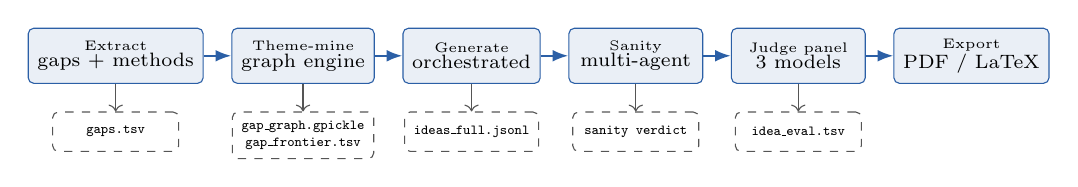
\begin{tikzpicture}[
      node distance=0.35cm and 0.35cm,
      every node/.style={font=\tiny},
      stage/.style={rectangle, draw=accent, fill=accent!10, rounded corners=2pt,
                    minimum width=1.7cm, minimum height=0.7cm, align=center},
      artifact/.style={rectangle, draw=muted, dashed, rounded corners=2pt,
                       minimum width=1.6cm, minimum height=0.5cm, align=center,
                       font=\tiny\ttfamily},
      arr/.style={-{Latex[length=2mm]}, draw=accent, thick},
    ]
    \node[stage] (extract) {Extract \\ \scriptsize gaps + methods};
    \node[stage, right=of extract] (theme)   {Theme-mine \\ \scriptsize graph engine};
    \node[stage, right=of theme]   (gen)     {Generate \\ \scriptsize orchestrated};
    \node[stage, right=of gen]     (sanity)  {Sanity \\ \scriptsize multi-agent};
    \node[stage, right=of sanity]  (judge)   {Judge panel \\ \scriptsize 3 models};
    \node[stage, right=of judge]   (export)  {Export \\ \scriptsize PDF / LaTeX};

    \draw[arr] (extract) -- (theme);
    \draw[arr] (theme)   -- (gen);
    \draw[arr] (gen)     -- (sanity);
    \draw[arr] (sanity)  -- (judge);
    \draw[arr] (judge)   -- (export);

    \node[artifact, below=of extract] (a1) {gaps.tsv};
    \node[artifact, below=of theme]   (a2) {gap\_graph.gpickle \\ gap\_frontier.tsv};
    \node[artifact, below=of gen]     (a3) {ideas\_full.jsonl};
    \node[artifact, below=of sanity]  (a4) {sanity verdict};
    \node[artifact, below=of judge]   (a5) {idea\_eval.tsv};

    \draw[->,muted] (extract) -- (a1);
    \draw[->,muted] (theme)   -- (a2);
    \draw[->,muted] (gen)     -- (a3);
    \draw[->,muted] (sanity)  -- (a4);
    \draw[->,muted] (judge)   -- (a5);
  \end{tikzpicture}

  \vspace{0.5em}
  \scriptsize Five sequential stages. Each writes an artifact downstream stages depend on.\\
  Multi-agent components: \textbf{generation orchestrator}, \textbf{sanity stage}, \textbf{judge panel}.
\end{frame}

% ---------------------------------------------------------------------

\section{v1: what existed and what was wrong}

\begin{frame}{v1 architecture}
  \begin{columns}[T]
    \column{0.55\textwidth}
      \textbf{Stages}
      \begin{itemize}
        \item \filename{extract-text} - PDF $\to$ text
        \item \filename{extract-sections} - regex-based Limitations / Future Work
        \item \filename{extract-gaps} - LLM, verbatim sentences
        \item \filename{theme-mine} - KMeans / HDBSCAN $\to$ centroid bridge pairs
        \item \filename{generate-ideas} - synthesiser + critic loop + judge panel
      \end{itemize}

    \column{0.45\textwidth}
      \textbf{Strengths}
      \begin{itemize}
        \item Verbatim provenance.
        \item Working multi-agent critic/judge stack.
        \item MCP server exposes the corpus to Claude Desktop.
      \end{itemize}
  \end{columns}
\end{frame}

\begin{frame}{v1 limits, in order of severity}
  \begin{enumerate}
    \item \alert{Clustering is the wrong primitive.}\\
      Single-membership partition over generic \texttt{all-MiniLM-L6-v2}
      embeddings. ``Bridge pairs'' computed centroid-to-centroid -
      averaging away exactly the gaps that bridge themes.
    \item \alert{No empirical sanity signal.}\\
      Judges score on text alone. Vague but ``novel-sounding'' ideas
      score well. No falsifiability requirement; no toy experiment.
    \item \alert{Section type lost mid-pipeline.}\\
      \filename{sections.py} detects \texttt{limitations} / \texttt{future\_work} /
      \texttt{discussion} but \filename{openai\_gaps.py} drops the label
      before writing \filename{gaps.tsv}.
  \end{enumerate}
\end{frame}

\begin{frame}{Why clustering hurts novelty specifically}
  \begin{itemize}
    \item HDBSCAN routes a chunk of gaps to \texttt{cluster\_id = -1} (noise).
      These are silently discarded.
    \item Tiny clusters (1-2 gaps from one paper) maximise
      \texttt{type\_complementarity} $\to$ inflate centroid bridge\_score.
    \item \texttt{peak(sim, 0.45)} is a hand-picked constant - never validated against the corpus.
    \item Cluster labels are LLM-generated from the first 8 sentences -
      non-deterministic across runs.
    \item \textbf{The deeper issue:} novel ideas live in the \emph{tails}, and clustering
      smooths the tails by design.
  \end{itemize}
\end{frame}

% ---------------------------------------------------------------------

\section{v2: five coordinated fixes}

\begin{frame}{Five PRs, shipped in order}
  \begin{table}\centering\scriptsize
    \begin{tabular}{@{}lllr@{}}
      \toprule
      PR & Goal & Risk & New tests \\
      \midrule
      1 & Propagate \texttt{section\_type} into \filename{gaps.tsv}                  & Low    & 7  \\
      2 & \texttt{falsifiable\_prediction} + \texttt{named\_baseline} gate           & Low    & 14 \\
      3 & Multi-agent experimental sanity stage                                       & Medium & 19 \\
      4 & Gap graph engine + \texttt{frontier} mode + MCP tools                       & Medium & 12 \\
      5 & Flip default to \flag{--method graph}; add \texttt{leiden\_graph} bench    & Low    & 1  \\
      \midrule
      \textbf{Total} &                                                                 &        & \textbf{53} \\
      \bottomrule
    \end{tabular}
  \end{table}

  \vspace{1em}
  \begin{itemize}
    \item Test count: 124 $\to$ 179 (+55) -- every PR ships with its own tests.
    \item Each PR keeps the pipeline runnable on its own; MCP backward compat preserved throughout.
    \item Defaults flipped only at the end, after head-to-head bench validation.
  \end{itemize}
\end{frame}

% ---------------------------------------------------------------------

\subsection{PR-1: section\_type propagation}

\begin{frame}[fragile]{PR-1: a latent bug fix the graph needs}
  \begin{itemize}
    \item \filename{sections.py} already classifies each section
      (\texttt{limitations} / \texttt{future\_work} / \texttt{discussion}
      / \texttt{fallback} / \texttt{tail}).
    \item The label is consumed at extraction time to prioritise input, then \alert{discarded}.
    \item \texttt{gaps.tsv} schema before:\\
      \scriptsize\texttt{(id, gap\_type, gap\_sentence, paragraph\_text, confidence)}
    \item \texttt{gaps.tsv} schema after:\\
      \scriptsize\texttt{(id, gap\_type,~\textbf{section\_type},~gap\_sentence, paragraph\_text, confidence)}
  \end{itemize}
  \vspace{0.5em}
  \textbf{Why this matters for v2:}
  \begin{itemize}
    \item The gap graph uses \texttt{section\_type} as an \emph{edge feature}.
    \item Critic and judge prompts see it as context -
      gaps from \texttt{future\_work} carry a different signal than from \texttt{limitations}.
    \item Backward-compat: \texttt{clean\_gaps} tolerates missing column - older
      \filename{gaps.tsv} files keep loading.
  \end{itemize}
\end{frame}

% ---------------------------------------------------------------------

\subsection{PR-2: falsifiability + named-baseline gate}

\begin{frame}[fragile]{PR-2: forcing falsifiability into the schema}
  Two new \emph{required} fields on every generated idea:
  \begin{lstlisting}
"falsifiable_prediction": "string with a QUANTITATIVE threshold,
                            e.g. >=5pp F1 gain vs RoBERTa-base on MNLI",
"named_baseline":         "a specific prior method/paper; never
                            'TBD', 'none', or 'no baseline'",
  \end{lstlisting}

  \begin{itemize}
    \item Schema is \texttt{strict=True}. The critic flags missing/weak versions
      as \emph{specificity} issues.
    \item \texttt{revise\_idea} now copy-forwards prior values if the revisor
      drops them (Claude/Gemini sometimes do).
    \item \texttt{evaluation.\_falsifiability\_gate} produces a boolean column
      on the eval TSV.
  \end{itemize}
  \vspace{0.3em}
  \alert{Effect:} the ``looks novel because vague'' failure mode is
  syntactically eliminated. A vague idea can't be written down.
\end{frame}

\begin{frame}[fragile]{The gate, in code}
  \begin{lstlisting}
_NUMERIC_RE = re.compile(
    r"(>=|<=|>|<|>=|<=)|"
    r"(\d+\.?\d*|\.\d+)\s*(%|pp|x||percent|points?|fold|sd)?",
    re.IGNORECASE,
)
_BAD_BASELINE_TOKENS = {"", "none", "n/a", "na", "tbd", "no baseline", ...}

def _falsifiability_gate(idea: dict) -> bool:
    pred = str(idea.get("falsifiable_prediction") or "").strip()
    base = str(idea.get("named_baseline") or "").strip()
    if not pred or not base:                  return False
    if base.lower() in _BAD_BASELINE_TOKENS:    return False
    return bool(_NUMERIC_RE.search(pred))
  \end{lstlisting}

  \scriptsize Surfaces as \texttt{falsifiability\_gate\_passed} in both single-judge and panel TSVs.
\end{frame}

% ---------------------------------------------------------------------

\subsection{PR-3: multi-agent experimental sanity stage}

\begin{frame}{PR-3: the central novelty of the thesis}
  \begin{itemize}
    \item Sits between the critic loop and the judge panel.
    \item Eleven agents, four phases, genuine deliberation -
      not a three-step pipeline.
    \item Experiment size is decided \emph{per idea} by the agents themselves
      (Tier 0--3), not capped at a fixed line count.
    \item Hard verdict constraints enforced \emph{after} the LLM call -
      schema validators, not just prompt language.
  \end{itemize}

  \vspace{0.5em}
  \alert{Hypothesis:} the ``looks novel because never executed'' failure
  mode is killed by forcing every accepted idea through a falsifiable
  experimental protocol.
\end{frame}

\begin{frame}{Phase architecture}
  \centering
  \scriptsize
  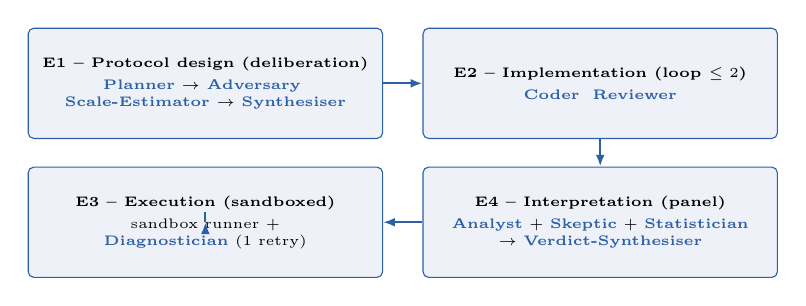
\begin{tikzpicture}[
      node distance=0.35cm and 0.5cm,
      every node/.style={font=\tiny, align=center},
      phase/.style={rectangle, draw=accent, fill=accent!8, rounded corners=2pt,
                    minimum width=4.5cm, minimum height=1.4cm},
      arr/.style={-{Latex[length=1.5mm]}, draw=accent, thick},
    ]
    \node[phase] (e1) {\textbf{E1 -- Protocol design (deliberation)}\\[2pt]
                       \agent{Planner} $\to$ \agent{Adversary} $\rightleftarrows$ \\
                       \agent{Scale-Estimator} $\to$ \agent{Synthesiser}};
    \node[phase, right=of e1] (e2) {\textbf{E2 -- Implementation (loop $\leq 2$)}\\[2pt]
                       \agent{Coder} $\rightleftarrows$ \agent{Reviewer}};

    \node[phase, below=of e1] (e3) {\textbf{E3 -- Execution (sandboxed)}\\[2pt]
                       sandbox runner +\\ \agent{Diagnostician} (1 retry)};
    \node[phase, below=of e2] (e4) {\textbf{E4 -- Interpretation (panel)}\\[2pt]
                       \agent{Analyst} + \agent{Skeptic} + \agent{Statistician}\\
                       $\to$ \agent{Verdict-Synthesiser}};

    \draw[arr] (e1) -- (e2);
    \draw[arr] (e2) -- (e2 |- e4.north);
    \draw[arr] (e4) -- (e3);
    \draw[arr] (e3) -- (e1 |- e3.east);
  \end{tikzpicture}

  \vspace{0.7em}
  \footnotesize
  Sample fan-out per phase varies (E1 four roles, E2 a coder/reviewer loop, E4 three independent assessors before synthesis).
  Agents on different models so disagreement is real.
\end{frame}

\begin{frame}{Tiered experiment sizing}
  \scriptsize
  \begin{table}\centering
    \begin{tabular}{@{}l p{5cm} r r@{}}
      \toprule
      Tier & Description & Code size & Wall budget \\
      \midrule
      0 & Untestable in a code sandbox (humans / proprietary data / hardware) & 0 & 0 s   \\
      1 & Smoke test on toy data; directional check                          & $\sim$30 LOC  & 10 s  \\
      2 & Synthetic controlled benchmark with $\geq 3$ seeds + baseline       & $\sim$80--200 LOC & 90 s  \\
      3 & Mini-real on a small public dataset, proper splits + stats         & $\sim$200--500 LOC & 600 s \\
      \bottomrule
    \end{tabular}
  \end{table}

  \vspace{1em}
  \begin{itemize}
    \item \flag{--sanity-budget \{smoke, benchmark, full\}} caps the maximum
      tier the Scale-Estimator may choose. Default \texttt{benchmark} (tier 2).
    \item Tier 0 is the honest escape hatch: ``cannot test this here.''
    \item Scale-Estimator's tier is \emph{hard-clamped} after the LLM call -
      not trusted to obey the budget on prompt language alone.
  \end{itemize}
\end{frame}

\begin{frame}[fragile]{Hard verdict constraints (enforced in code)}
  Schema language tells the LLM the rules. The validator then enforces them:
  \begin{lstlisting}
if tier == 0:
    verdict["sanity_supported"] = "untestable"
elif not ran_to_completion:
    if verdict["sanity_supported"] == "yes":
        verdict["sanity_supported"] = "inconclusive"
elif confound >= 0.6 and verdict["sanity_supported"] == "yes":
    verdict["sanity_supported"] = "partial"
elif power == "insufficient" and verdict["sanity_supported"] == "yes":
    verdict["sanity_supported"] = "partial"
  \end{lstlisting}

  \vspace{0.3em}
  \begin{itemize}
    \item Skeptic's \texttt{confound\_score} $\geq 0.6$ \emph{cannot} co-exist with verdict \texttt{yes}.
    \item Statistician's \texttt{insufficient} power \emph{cannot} co-exist with verdict \texttt{yes}.
    \item Disagreement between Skeptic and Analyst $\Rightarrow$ \texttt{inconclusive} is a valid output.
  \end{itemize}
\end{frame}

% ---------------------------------------------------------------------

\subsection{PR-4: gap graph engine}

\begin{frame}{PR-4: replace clustering with a multi-relational graph}
  \begin{itemize}
    \item Nodes: individual gap sentences (not cluster centroids).
    \item Edges: four relations encoding both semantic and provenance similarity.
    \item Communities (Leiden / Louvain) become a \emph{view} over the graph -
      written to \texttt{cluster\_id} for backward compat.
    \item Bridge pairs become \emph{edge-betweenness} - structural bridges,
      not centroid pairs.
    \item New: \texttt{frontier\_nodes} - gaps at community boundaries -
      the long-tail seeds HDBSCAN would discard.
  \end{itemize}
\end{frame}

\begin{frame}{Graph anatomy}
  \begin{columns}[T]
    \column{0.55\textwidth}
      \textbf{Four edge types}\\[0.3em]
      \scriptsize
      \begin{tabular}{@{}l p{4cm}@{}}
        \toprule
        Type & Predicate \\
        \midrule
        \texttt{semantic} & top-$k$ cosine $\geq$ threshold \\
        \texttt{paper}    & same \texttt{paper\_id} \\
        \texttt{section}  & same \texttt{section\_type}, cosine $\geq 0.3$ \\
        \texttt{method}   & bipartite, cosine $\in (0.3, 0.7)$ \\
        \bottomrule
      \end{tabular}
      \vspace{0.7em}
      \\
      \footnotesize Method nodes are tagged \texttt{bipartite=1} and \emph{excluded} from community detection.

    \column{0.4\textwidth}
      \centering
      \scriptsize
      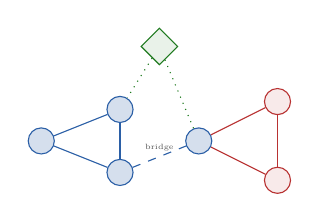
\begin{tikzpicture}[node distance=0.3cm, every node/.style={font=\tiny}]
        \node[circle, draw=accent, fill=accent!20, minimum size=4pt] (g1) at (0,0)   {};
        \node[circle, draw=accent, fill=accent!20, minimum size=4pt] (g2) at (1,0.4) {};
        \node[circle, draw=accent, fill=accent!20, minimum size=4pt] (g3) at (1,-0.4){};
        \node[circle, draw=accent, fill=accent!20, minimum size=4pt] (g4) at (2,0)   {};
        \node[circle, draw=warn,   fill=warn!10,  minimum size=4pt] (g5) at (3,0.5) {};
        \node[circle, draw=warn,   fill=warn!10,  minimum size=4pt] (g6) at (3,-0.5){};
        \node[diamond, draw=ok,    fill=ok!10,    minimum size=4pt] (m1) at (1.5,1.2){};

        \draw[-, accent]      (g1) -- (g2);
        \draw[-, accent]      (g1) -- (g3);
        \draw[-, accent]      (g2) -- (g3);
        \draw[-, accent, dashed] (g3) -- (g4) node[midway,above,muted,scale=0.55] {bridge};
        \draw[-, warn]        (g5) -- (g6);
        \draw[-, warn]        (g4) -- (g5);
        \draw[-, warn]        (g4) -- (g6);
        \draw[-, ok, dotted]  (m1) -- (g2);
        \draw[-, ok, dotted]  (m1) -- (g4);
      \end{tikzpicture}
      \vspace{0.3em}\\
      \scriptsize Blue + red: gap communities.\\Green diamond: method node (bipartite).
  \end{columns}
\end{frame}

\begin{frame}[fragile]{Three operators replace centroid clustering}
  \scriptsize
  \begin{lstlisting}
def build_gap_graph(gaps, embeddings, *, knn_k, sim_threshold,
                    methods=None, method_embeddings=None) -> nx.Graph

def detect_communities(G, *, resolution, seed) -> np.ndarray
    # Leiden via igraph+leidenalg if installed,
    # NetworkX Louvain fallback. Renumbers by (n_papers, n_items)
    # so cluster_ids are STABLE across runs.

def graph_bridge_pairs(G, community_ids, *, top_n) -> pd.DataFrame
    # edge-betweenness summed per (community_a, community_b),
    # normalised to [0, 1]. Same columns as legacy cluster_pairs.tsv.

def graph_individual_pairs(G, community_ids, gaps, *, top_n) -> pd.DataFrame
    # one row per gap-gap bridge -- the REAL bridges that centroid
    # pair scoring averages away.

def frontier_nodes(G, community_ids, gaps, *, top_n) -> pd.DataFrame
    # boundary gaps: low intra-community degree, high neighbour-community
    # diversity. New `frontier` generation mode seeds from these.
  \end{lstlisting}
\end{frame}

% ---------------------------------------------------------------------

\subsection{PR-5: flip defaults + bench}

\begin{frame}{PR-5: making the new architecture the default}
  \begin{itemize}
    \item \flag{theme-mine --method} default flipped from \texttt{kmeans} $\to$ \texttt{graph}.
    \item \flag{--embed-model} help text now documents \texttt{malteos/scincl}
      and \texttt{allenai/specter2\_base} as science-tuned alternatives -
      but default kept as \texttt{all-MiniLM-L6-v2} so first runs don't
      surprise users with a large model download.
    \item \texttt{clustering\_bench.fit\_clusters} gains a \texttt{leiden\_graph}
      entry. The existing plot harness (\filename{clustering\_bench\_plots.py})
      produces a head-to-head figure across:
      \begin{itemize}
        \scriptsize
        \item KMeans, Agglomerative, HDBSCAN, HDBSCAN+UMAP, BERTopic, \alert{leiden\_graph}.
      \end{itemize}
    \item Legacy \texttt{cluster\_embeddings} + \texttt{build\_cluster\_pairs}
      \emph{not} removed - they remain the \flag{--method kmeans} implementation
      with regression tests.
  \end{itemize}
\end{frame}

% ---------------------------------------------------------------------

\section{Walkthrough}

\begin{frame}{End-to-end run -- placeholder slides}
  The remaining walkthrough slides are \alert{templates}. They will be
  filled in once the pipeline produces an idea worth showing:
  \begin{itemize}
    \item Generated idea content (title, RQ, method, evaluation plan)
    \item v2 schema fields populated (\texttt{falsifiable\_prediction},
      \texttt{named\_baseline})
    \item Sanity-stage verdict + tier
    \item Judge-panel scores + agreement
    \item Honest critique of the result
  \end{itemize}
\end{frame}

\begin{frame}{Walkthrough -- the idea (template)}
  \todoslide{drop in the final idea title + research question + method sketch}

  \begin{itemize}
    \item \textbf{Title:} \texttt{TODO}
    \item \textbf{Research question:} \texttt{TODO}
    \item \textbf{Method sketch:} \texttt{TODO}
    \item \textbf{Evaluation plan:} \texttt{TODO}
    \item \textbf{Expected contribution:} \texttt{TODO}
  \end{itemize}
\end{frame}

\begin{frame}{Walkthrough -- v2 schema fields (template)}
  \todoslide{paste the falsifiable\_prediction + named\_baseline from ideas.tsv}

  \begin{itemize}
    \item \texttt{falsifiable\_prediction}: \alert{TODO -- must include a quantitative threshold}
    \item \texttt{named\_baseline}: \alert{TODO -- must name a specific prior method}
    \item \texttt{falsifiability\_gate\_passed}: \alert{TRUE / FALSE}
  \end{itemize}
\end{frame}

\begin{frame}{Walkthrough -- sanity-stage verdict (template)}
  \todoslide{paste the sanity\_* columns and 1--2 sentences of the trace}
  \begin{itemize}
    \item \texttt{sanity\_tier}: \alert{TODO}
    \item \texttt{sanity\_ran}: \alert{TODO}
    \item \texttt{sanity\_supported}: \alert{yes / partial / no / inconclusive / untestable}
    \item \texttt{sanity\_signal}: \alert{TODO} (0--1)
    \item \texttt{sanity\_confound\_score}: \alert{TODO} (0--1)
    \item Key trace excerpt: \alert{TODO}
  \end{itemize}
\end{frame}

\begin{frame}{Walkthrough -- judge panel + critique (template)}
  \todoslide{paste the panel breakdown across novelty / specificity / feasibility / grounding}

  \scriptsize
  \begin{tabular}{@{}l c c c c c c@{}}
    \toprule
    Judge & Novelty & Spec. & Feas. & Ground. & Composite & Agreement \\
    \midrule
    Claude Sonnet 4 & \texttt{?} & \texttt{?} & \texttt{?} & \texttt{?} & & \\
    GPT-4o          & \texttt{?} & \texttt{?} & \texttt{?} & \texttt{?} & & \\
    Gemini 2.5 Flash& \texttt{?} & \texttt{?} & \texttt{?} & \texttt{?} & & \\
    \midrule
    \textbf{Consensus} & \textbf{?} & \textbf{?} & \textbf{?} & \textbf{?} & \textbf{?} & \textbf{?} \\
    \bottomrule
  \end{tabular}

  \vspace{0.7em}
  \normalsize
  \alert{TODO}: 1--2 sentences of honest critique from the consensus\_critique field.
\end{frame}

% ---------------------------------------------------------------------

\section{What this contributes}

\begin{frame}{Thesis contributions}
  \begin{enumerate}
    \item \textbf{Multi-relational gap graph} as a primitive for research-idea
      synthesis - replaces single-membership clustering. Treats ``bridge''
      as a graph concept, not a partition concept.
    \item \textbf{Frontier-mode generation} - mines novelty seeds from
      community boundaries (the gaps clustering throws away).
    \item \textbf{Multi-agent experimental sanity stage} with tiered
      claim-conditioned experiment sizing and hard post-LLM verdict
      constraints. Falsifiable, sandboxed, cost-bounded.
    \item \textbf{Falsifiability + named-baseline gate} on every generated
      idea - syntactically eliminates the vague-idea failure mode.
    \item \textbf{Open implementation:} 1 module per contribution, $\sim$3000 LOC,
      53 new tests, backward-compatible MCP interface.
  \end{enumerate}
\end{frame}

\begin{frame}{Limitations}
  \begin{itemize}
    \item \textbf{Sanity stage cost} - $\sim\$0.04$--$0.20$/idea with all
      agents on cheap models; higher with Sonnet for adversary/skeptic.
      Mitigated by the confidence + critic gate (only $\sim$30--40\% of ideas
      reach sanity).
    \item \textbf{Citation graph deferred to v2} - paper-A-cites-paper-B
      edges would be a strong additional signal but require an
      authenticated S2 prefetch and rate-limit handling.
    \item \textbf{Embedder still generic} by default - SciNCL / SPECTER2
      swap is documented but opt-in until the bench validates the metric lift.
    \item \textbf{Tier-3 runs} can blow batch throughput; current default
      caps at Tier 2 (\flag{--sanity-budget benchmark}).
    \item \textbf{Cluster/community labels are still LLM-generated} - some
      stochasticity across runs even after the renumbering trick.
  \end{itemize}
\end{frame}

\begin{frame}{Future work}
  \begin{itemize}
    \item Citation-graph edges + authenticated S2 prefetch.
    \item Active sanity revision: a failed sanity verdict re-enters the
      critic loop with the failure as new input.
    \item Heterogeneous communities including method nodes
      (bipartite community detection).
    \item Embedder ensembles (MiniLM + SciNCL late fusion).
    \item Idea-space coverage map: meta-cluster of \texttt{ideas.tsv} to
      surface white space in the idea distribution.
    \item Cross-run deduplication via content-addressed cache on
      \texttt{hash(research\_question)}.
  \end{itemize}
\end{frame}

\begin{frame}[standout]
  Thank you.\\[1em]
  \normalsize Questions?
\end{frame}

% =====================================================================
% Appendix: extra detail slides
% =====================================================================
\appendix

\begin{frame}{Appendix -- extra detail slides}
  \begin{itemize}
    \item Sanity-stage agent roles + default models
    \item Sandbox implementation: env, network block, memory cap
    \item Backward-compat artifacts (same TSV schemas)
    \item Graph reproducibility + community renumbering
    \item Frontier evidence selection
    \item CLI flag reference
    \item MCP tool surface
    \item Test count by PR
    \item Cost estimates
    \item Failure modes covered by the 11 agents
    \item Bench head-to-head: legacy vs graph
  \end{itemize}
\end{frame}

% ---------- A1 ----------
\begin{frame}{A1 -- The 11 sanity-stage agents}
  \scriptsize
  \begin{tabular}{@{}l l l@{}}
    \toprule
    Phase & Role & Default model \\
    \midrule
    E1 & Planner             & gpt-4.1-mini \\
       & Adversary           & claude-sonnet-4 \\
       & Scale-Estimator     & gpt-4.1-mini \\
       & Protocol-Synthesiser & claude-sonnet-4 \\
    \midrule
    E2 & Coder               & claude-sonnet-4 \\
       & Reviewer            & gpt-4.1-mini \\
    \midrule
    E3 & Sandbox runner      & (subprocess; not an LLM) \\
       & Diagnostician       & gpt-4.1-mini \\
    \midrule
    E4 & Analyst             & gpt-4.1-mini \\
       & Skeptic             & claude-sonnet-4 \\
       & Statistician        & gpt-4.1-mini \\
       & Verdict-Synthesiser & claude-sonnet-4 \\
    \bottomrule
  \end{tabular}

  \vspace{0.5em}
  \footnotesize Cheap fast model on Planner/Reviewer/Analyst/Statistician;
  stronger reasoner on Adversary/Skeptic/Coder/Synthesisers. All overridable via
  \flag{--sanity-models}.
\end{frame}

% ---------- A2 ----------
\begin{frame}[fragile]{A2 -- Sandbox env + network block}
  \scriptsize
  \begin{itemize}
    \item Subprocess: \texttt{[sys.executable, "-I", "-S", script]} -
      isolated mode, no site, fresh tempdir cwd.
    \item Env: deliberately minimal:
      \begin{lstlisting}
sandbox_env = {"PYTHONIOENCODING": "utf-8", "PATH": ""}
if sys.platform == "win32":
    for k in ("SYSTEMROOT", "WINDIR", "TEMP", "TMP", "COMSPEC"):
        v = os.environ.get(k)
        if v: sandbox_env[k] = v
      \end{lstlisting}
    \item Network block: prepended to every script, subclasses
      \texttt{socket.socket} instead of replacing it (so \texttt{ssl}
      keeps importing):
      \begin{lstlisting}
_orig_socket = socket.socket
class _BlockedSocket(_orig_socket):
    def connect(self, *a, **k):
        raise OSError("network disabled by sandbox")
socket.socket = _BlockedSocket
      \end{lstlisting}
    \item Memory cap on POSIX via \texttt{preexec\_fn} + \texttt{resource.setrlimit};
      Windows falls back to wall-clock kill (\texttt{TimeoutExpired}).
  \end{itemize}
\end{frame}

% ---------- A3 ----------
\begin{frame}{A3 -- Backward-compat artifacts (same schemas)}
  \scriptsize
  Even with \flag{--method graph}, the following artifacts keep their
  legacy column schemas so MCP + generation modes work unchanged:
  \vspace{0.5em}
  \begin{tabular}{@{}l p{8cm}@{}}
    \toprule
    File & Columns (after PR-4, identical to v1) \\
    \midrule
    \texttt{gaps\_with\_clusters.tsv} & \texttt{id, gap\_type, section\_type, gap\_sentence, paragraph\_text, confidence, cluster\_id} \\
    \texttt{cluster\_labels.tsv}      & \texttt{cluster\_id, theme\_label, keywords} \\
    \texttt{cluster\_summary.tsv}     & \texttt{cluster\_id, n\_items, n\_papers, avg\_conf, theme\_label, examples} \\
    \texttt{cluster\_pairs.tsv}       & \texttt{cluster\_a, cluster\_b, label\_a, label\_b, cosine\_sim, paper\_overlap, type\_complementarity, bridge\_score} \\
    \midrule
    \textbf{New artifacts} & \\
    \texttt{gap\_graph.gpickle}       & pickled NetworkX graph \\
    \texttt{gap\_pairs.tsv}           & individual-gap bridges \\
    \texttt{gap\_frontier.tsv}        & frontier gaps for frontier mode \\
    \bottomrule
  \end{tabular}
\end{frame}

% ---------- A4 ----------
\begin{frame}{A4 -- Graph reproducibility}
  \begin{itemize}
    \item Community IDs are renumbered post-detection by
      \texttt{(n\_papers desc, n\_items desc, raw\_id asc)}.
    \item Same corpus + same seed $\Rightarrow$ identical \texttt{cluster\_id}
      integers across runs.
    \item Tested explicitly:
      \texttt{test\_detect\_communities\_is\_reproducible} and
      \texttt{test\_detect\_communities\_renumbers\_largest\_first}.
    \item Avoids the legacy KMeans + LLM-label problem where
      \texttt{cluster\_id=3} could be ``vision'' one day and ``RL'' the next.
  \end{itemize}
\end{frame}

% ---------- A5 ----------
\begin{frame}[fragile]{A5 -- Frontier evidence selection}
  No new bookkeeping; relies on the structure of embedding space:
  \begin{lstlisting}
def _frontier_evidence(gaps, embeddings, seed_idx, *, k_evidence=4):
    """Build evidence for a frontier gap: the seed gap + its
    (k-1) nearest neighbours by cosine. Because the seed sits on a
    community boundary, the neighbours naturally span the bridging
    clusters -- no extra bookkeeping needed."""
    seed_emb = embeddings[seed_idx]
    sims = embeddings @ seed_emb
    sims[seed_idx] = -np.inf
    order = np.argsort(-sims)[:k_evidence - 1]
    pick = np.concatenate(([seed_idx], order)).astype(int)
    return gaps.iloc[pick].reset_index(drop=True)
  \end{lstlisting}
  \footnotesize Frontier mode then routes through the within-mode synthesis
  prompt because the evidence list is a single set (not a paired
  bridge). The bridge structure falls out of the seed's geometry, not the prompt.
\end{frame}

% ---------- A6 ----------
\begin{frame}{A6 -- CLI flags reference (new in v2)}
  \scriptsize
  \begin{tabular}{@{}p{5.6cm} p{6.5cm}@{}}
    \toprule
    Flag & Effect \\
    \midrule
    \flag{theme-mine --method graph$|$kmeans}        & default: graph (PR-5) \\
    \flag{--knn-k}                                    & top-k semantic neighbours per gap \\
    \flag{--sim-threshold}                            & min cosine for a semantic edge \\
    \flag{--leiden-resolution}                        & community resolution \\
    \flag{--frontier-top-n}                           & rows to write to gap\_frontier.tsv \\
    \midrule
    \flag{generate-ideas --mode frontier}             & seed from frontier gaps \\
    \flag{--orchestrate-mode frontier}                & frontier inside the orchestrator \\
    \flag{--sanity} / \flag{--no-sanity}              & enable the multi-agent sanity stage \\
    \flag{--sanity-budget \{smoke,bench,full\}}       & cap max tier the Scale-Estimator may choose \\
    \bottomrule
  \end{tabular}
\end{frame}

% ---------- A7 ----------
\begin{frame}{A7 -- MCP tool surface (post-PR-4)}
  \scriptsize
  \begin{tabular}{@{}l l@{}}
    \toprule
    Tool & Effect \\
    \midrule
    \texttt{list\_themes}            & every cluster, label, size \\
    \texttt{get\_theme(cluster\_id)} & one theme: label, keywords, papers, gaps \\
    \texttt{get\_evidence(cluster\_id, k)} & k diverse evidence rows \\
    \texttt{retrieve\_methods(cluster\_id)} & sweet-spot method statements \\
    \texttt{search\_prior\_art(query)} & Semantic Scholar search \\
    \texttt{score\_novelty(title, rq)} & 1 -- max cosine vs S2 hits \\
    \texttt{check\_evidence\_overlap(used, fed)} & hallucination check \\
    \texttt{list\_ideas} / \texttt{get\_idea} / \texttt{save\_idea} & idea library CRUD \\
    \alert{\texttt{list\_frontier(top\_n)}}   & \alert{PR-4: top frontier gaps} \\
    \alert{\texttt{list\_gap\_pairs(top\_n)}} & \alert{PR-4: top structural bridges} \\
    \bottomrule
  \end{tabular}

  \vspace{0.6em}
  \footnotesize Existing tools unchanged. New tools degrade to empty result
  if the graph artifacts haven't been produced.
\end{frame}

% ---------- A8 ----------
\begin{frame}{A8 -- Tests added per PR}
  \begin{table}\centering\scriptsize
    \begin{tabular}{@{}l l r r@{}}
      \toprule
      PR & Test file & New tests & Cumulative \\
      \midrule
      1 & \texttt{test\_openai\_gaps.py}, \texttt{test\_theme\_mining.py}, \texttt{test\_sections.py} & 7  & 131 \\
      2 & \texttt{test\_evaluation.py}, \texttt{test\_openai\_ideas.py}, \texttt{test\_agents.py}    & 14 & 145 \\
      3 & \texttt{test\_sanity.py}                                                                     & 19 & 164 \\
      4 & \texttt{test\_gap\_graph.py}                                                                 & 12 & 176 \\
      5 & \texttt{test\_gap\_graph.py} (bench entry)                                                   & 1  & 177 \\
      \midrule
      Pre-v2 baseline & -- & -- & 124 \\
      \textbf{Post-v2} & & \textbf{+55} & \textbf{179} \\
      \bottomrule
    \end{tabular}
  \end{table}

  \vspace{0.5em}
  \footnotesize Tests cover sandbox semantics (network block, timeout, env), schema
  parity with legacy, agent deliberation (tier clamp, reviewer loop,
  verdict downgrade), and reproducibility (seeded community IDs).
\end{frame}

% ---------- A9 ----------
\begin{frame}{A9 -- Cost estimates}
  Per accepted idea, with default models:
  \scriptsize
  \begin{table}\centering
    \begin{tabular}{@{}l l r r@{}}
      \toprule
      Stage & LLM calls & USD (cheap mix) & USD (Sonnet-heavy) \\
      \midrule
      Synth + critic loop (up to 2) & $\sim$5 & 0.01--0.03 & 0.05--0.10 \\
      Sanity E1 (4 agents)          & 4       & 0.005--0.02 & 0.02--0.04 \\
      Sanity E2 (1--2 rounds)       & 2--4    & 0.01--0.03  & 0.04--0.10 \\
      Sandbox subprocess            & 0       & 0           & 0          \\
      Sanity E4 (4 agents)          & 4       & 0.005--0.02 & 0.02--0.04 \\
      Judge panel (3 judges)        & 3       & 0.01--0.03  & 0.05--0.08 \\
      \midrule
      \textbf{Total per idea (tier 1, smoke)} & $\sim$18 & \textbf{0.04--0.10} & \textbf{0.15--0.30} \\
      \textbf{Total per idea (tier 2, benchmark)} & $\sim$20 & \textbf{0.05--0.15} & \textbf{0.20--0.50} \\
      \bottomrule
    \end{tabular}
  \end{table}

  \vspace{0.5em}
  \footnotesize Gate filters $\sim$60\% of ideas before sanity, so batch costs
  are lower than per-idea totals suggest. Cache hits on
  \texttt{(idea\_id, protocol)} cut iteration cost to E4 only ($\sim$0.04/idea).
\end{frame}

% ---------- A10 ----------
\begin{frame}{A10 -- Failure modes the 11 agents catch}
  \scriptsize
  \begin{table}\centering
    \begin{tabular}{@{}l l@{}}
      \toprule
      Failure mode                                  & Caught by \\
      \midrule
      Tier too high for the claim                   & Scale-Estimator clamp + Adversary attack \\
      Reviewer rubber-stamps the code               & Mitigation: hard-cap loop at 2 rounds; log rejection rate \\
      Coder writes non-deterministic code           & Coder system prompt: seeded RNG, n\_seeds in protocol \\
      Tier 3 run blows the wall budget              & \flag{--sanity-budget} caps; default = benchmark = tier 2 \\
      Diagnostician hallucinates a fix              & Hard cap: 1 retry; E4 sees the failure either way \\
      Skeptic raises strong confounds, LLM says yes & Hard schema rule: confound $\geq 0.6 \Rightarrow$ max ``partial'' \\
      Single-seed run                               & Statistician $\Rightarrow$ \texttt{power=insufficient} $\Rightarrow$ max ``partial'' \\
      Network leak from generated code              & Pre-pended \texttt{socket.socket} subclass override \\
      Verdict-Synthesiser conflicts with the panel  & Disagreement $\Rightarrow$ \texttt{inconclusive} (a valid outcome) \\
      \bottomrule
    \end{tabular}
  \end{table}
\end{frame}

% ---------- A11 ----------
\begin{frame}{A11 -- Five-commit history}
  \scriptsize
  \begin{tabular}{@{}l l l@{}}
    \toprule
    Commit & PR & Subject \\
    \midrule
    \texttt{2737886} & 1 & \texttt{feat(extraction): propagate section\_type into gaps.tsv} \\
    \texttt{b509ab1} & 2 & \texttt{feat(generation): falsifiability + named-baseline gate on ideas} \\
    \texttt{f1fb61d} & 3 & \texttt{feat(sanity): multi-agent experimental sanity stage with tiered budget} \\
    \texttt{08034df} & 4 & \texttt{feat(graph): multi-relational gap graph replaces clustering as the primitive} \\
    \texttt{4116f20} & 5 & \texttt{feat(graph): flip theme-mine default to --method graph; add leiden\_graph bench clusterer} \\
    \bottomrule
  \end{tabular}

  \vspace{1em}
  \footnotesize Five reviewable PRs; each ships its own tests; no
  mid-migration breakage; pipeline runnable after every commit.
\end{frame}

% ---------- A12 ----------
\begin{frame}{A12 -- Why this is multi-agent, not a chain}
  A chain has handoffs. A multi-agent system has deliberation. The
  sanity stage is genuinely the latter:
  \begin{itemize}
    \item \textbf{E1} - \agent{Planner} drafts; \agent{Adversary} attacks on
      a \emph{different model}; \agent{Scale-Estimator} arbitrates;
      \agent{Synthesiser} merges. None of the four can unilaterally
      override the others' decisions.
    \item \textbf{E2} - true loop. Reviewer can reject. The Coder rewrites in
      response. Either may ``win.''
    \item \textbf{E4} - independent panel: \agent{Analyst} states facts,
      \agent{Skeptic} argues alternatives, \agent{Statistician} imposes
      a numeric reality check. \agent{Verdict-Synthesiser} \emph{must}
      reconcile disagreement and is \emph{allowed} to return \texttt{inconclusive}.
    \item Disagreement is data, not error.
  \end{itemize}
\end{frame}

\end{document}
